\section{Mountain car}\label{experiment:mountaincar}

With the Mountain car problem, a car is supposed to drive up a mountain that is too steep for the car's engine. To achieve is to build up momentum to reach the target as fast as possible given the position $p$ and velocity $v$ of the car.

% todo hein "o-dimensional state space s = (r, ˙r)"

\begin{figure}[ht]
	\centering
  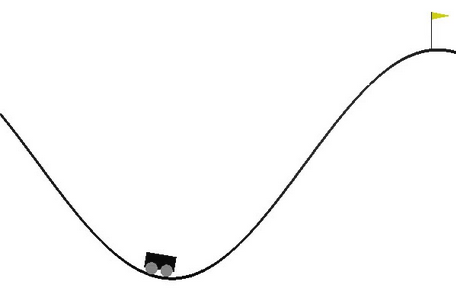
\includegraphics[scale=0.6]{img/MTC/MTC_experiment.PNG}
	\caption{A possible starting position in MC}
	\label{img:mtc_experiment}
\end{figure}

In the discrete version of MC there are three possible actions:

\begin{tabular}{ll}
\hline 
Num & Action\tabularnewline
\hline 
0 & push left\tabularnewline
1 & no push\tabularnewline
2 & push right\tabularnewline
\hline 
\end{tabular}

The problem was first introduced in 1990 \cite{mountaincarOriginal} and has since become a widely used RL benchmark.

\begin{tabular}{|c|c|c|c|}
\hline 
Num & Observarion & Min & Max\tabularnewline
\hline 
\hline 
0 & position & -1.2 & 0.06\tabularnewline
\hline 
1 & velocity & -0.07 & 0.07\tabularnewline
\hline 
\end{tabular}

\begin{tabular}{|c|c|}
\hline 
Num & Action\tabularnewline
\hline 
\hline 
0 & push left\tabularnewline
\hline 
1 & no push\tabularnewline
\hline 
2 & push right\tabularnewline
\hline 
\end{tabular}






\subsection{Learning goals on the way to the perfect solution }

Attempts to reduce the distance to the target by accelerating in its direction are quickly recognized as unsuccessful. 
In order to reach the target at all, the agent must learn to gain momentum with the help of the counter slope. This can be achieved, for example, with the "simple" heuristic of always accelerating in the direction in which one is currently moving.

This way you always reach your goal, but there is still plenty of room for optimization.
These are:
\begin{itemize}
\item Turn back early: To reach the goal, you don't have to take the maximum momentum. If you turn back earlier, a lot of time can be saved.
\item Discard Action 1 "Do nothing": Doing nothing makes no sense in principle - speed is lost when taking a swing and when turning around, instead of doing nothing two consecutive times, you could normally accelerate in the opposite direction.
\item Number of necessary swings: Depending on starting position of experiment, target can be reached by two or three starts. The agent must therefore decide in the initial state already in which direction to start. A safety buffer does not have to be taken into account, since all other states are deterministic.
\end{itemize}

\paragraph{Problems}

The initial state is a major problem for regression analyses because, despite its crucial role, it occurs only once in the data set. For this reason, there are sometimes large differences in performance when testing the agents.
Just past is also beside the point. Some Sarsa runs end with very tight finishes. Some runs of the trained agents are unfortunately not lucky and have to turn back shortly before the finish.

The SARSA approach was chosen because it was the fastest that could solve mountain car well. However, this meant that little was explored in the learning process and often there are wrong decisions that 
   but there's still a lot of air up there. Very easy to learn that the goal can be achieved with less momentum and you can turn with 

funfact:
cartvel < 0 then 0 else 2
cartvel <= 0 then 0 else 2 

Reverse early

This simple policy can further be improved, where the most efficient way is probably by reversing early on the opposite side. 

\paragraph{Close-form preset policy}

In \cite{xiao2019}, a close-form preset policy was proposed, defining a lower and upper bound  for the car to determine the actions.
\begin{figure}
    \centering
    
    \begin{lstlisting}
    push right, when:\\
    $min(-0.09(position + 0.25)^2+0.03, 0.3(position + 0.09)^4-0.008)\\
    \leq velocity \leq \\
    (-0.07(position + 0.38)^2 + 0.07)$\\
    push left instead
    \end{lstlisting}
    \caption{Pseudocode for getting first layer of modifiable nodes}
    \label{code:MC-agent:preset_policy}
\end{figure}

\paragraph{Real solution, optimal solution and expert abstraction}

As we will see and discuss in \ref{todo}, the first decision is most relevant for the optimal solution. The starting velocity is always 0, but depending on the starting position, you have to take three or four turns to reach the goal. For this purpose, another expert policy has been implemented, which explicitly emphasizes this state.


\subsection{Machine learning approach}

    
\begin{figure}[ht]
	\centering
  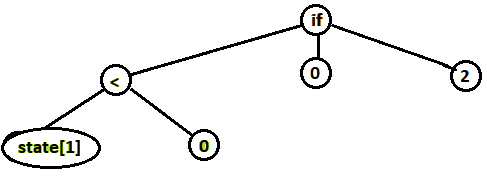
\includegraphics[scale=0.6]{img/MTC/mtc_simple_tree.png}
	\caption{Computational tree of the simplest program}
	\label{img:mtc_simple_tree}
\end{figure}

The only real requirement of the approach is that it performs better on average than the explainable approach and is based on a neural network. Conveniently, the gym-environment has a leaderboard containing the approaches that have been able to learn the fastest to create a policy that solves the problem in steps of less than $110$. \ref{mtc_leaderboards}
The approach chosen here is a SARSA procedure [TODO paper Sarsa? Approach?] with tiling that is able to learn a sufficient policy after 75 episodes with an average episode reward of $\approx-103.4$.

The same approach war also trained for 200 episodes but a better average result of $\approx-98.7$

\begin{tabular}{l l l}
  Agent   & Training episodes  & Average episode reward (100 runs) \\\hline
  Sarsa 75 &  75  &  -103.41 \tabularnewline
  Sarsa 200 &  200  &  -98.68 \tabularnewline
  Sarsa 1000 &  1000  &  -106.78 \tabularnewline
  Sarsa 10.000 &  10000  &  -109.31 \tabularnewline \hline
  Simple agent & ($<$) & -119.41 \tabularnewline
  Bad simple agent & ($<=$) & -129.62 \tabularnewline \hline
  Fix preset Policy & & -102.61 \tabularnewline
  
\end{tabular}


\noindent For this initial experiment, the black box is explicitly not , the way it works was deliberately not looked at in detail.

\paragraph{First evaluation} 

The ``simple'' policy reached the target with an average episode reward of $-119$ without fails very constantly. The average reward of the SARSA-agent is, with an average reward of $103$, outperforming the ``simple'' approach with about $14\%$.
A grain of salt however is, that the SARSA Approach seems to be relatively unstable, even causing the policy to almost fail to reach the target in 200 steps, as can be seen in \ref{img:MTC-heuristic-vs-sarsa-reward}. The reason for poor performance was not evaluated, even though it can be assumed that this is caused by uncommon starting states where not enough experience was made yet. [todo epsilon wert = 0?] 


\begin{figure}[ht]
	\centering
  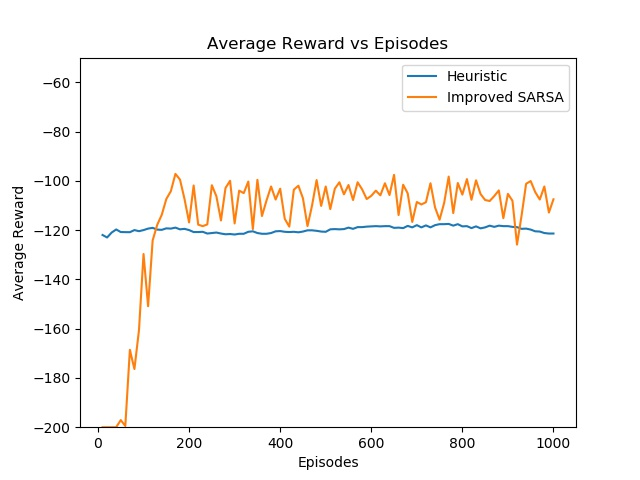
\includegraphics[scale=0.4]{img/MTC/MTC-heuristic_vs_sarsa-1000-10-average.jpg}
  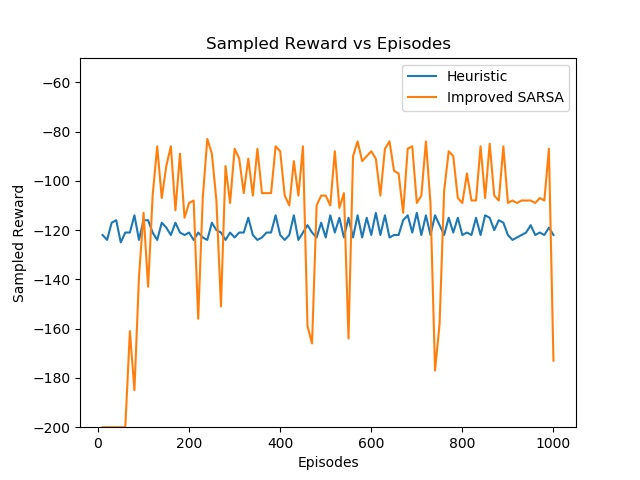
\includegraphics[scale=0.4]{img/MTC/MTC-heuristic_vs_sarsa-1000-10.jpg}
	\caption{SARSA implementation learns to outperform the heuristic on average}
	\label{img:MTC-heuristic-vs-sarsa-reward}
\end{figure}


    % TODO. Zeigen, wie RL nach einer Zeit besser als die Heuristik abschneidet
    % TODO: RL machen auch manchmal doofe Sachen. Zappeln im Reward, beispielsweise


    


\subsection{GP preparation}
The samples sample size of the data resulted from going through 15 complete runs of mountain car with the chosen SARSA-Approach. These runs were taken randomly and all observations and decisions were considered, resulting in about $2000$ samples. The data was then split into 80\% training and 20\% test data to verify the results.\\




\subsection{Missing action ``no push''}

Action ``no push'', even though it is possible, 

One aspect of ignoring all information from the black box was to create a mountain car core solution that does not allow it to stand still whereas the black box solution considered option '0' of not moving. This option was used in $134/2088$ samples, which is about $6.4\%$\\

[todo insert picture of the tree and/or the sarsa choices]\\
This is already a relatively large, categorical difference to the expert, which raises many questions.
Has this limitation perhaps already caused a gross error? Is the gp process affected by this?
This question is indeed difficult to answer. Action ``no push'' is in fact hardly relevant for solving the problem, since a quick turn around by reversing the acceleration is more efficient than doing nothing. This limitation is in fact an area of core logic of the expert program that precedes the SARSA approach. However, if this decision has not been made as the conclusion of an analysis, action ``no push'' may need to be reconsidered.
Thus, while this restriction is legitimate from a logical point of view, from a technical point of view it also causes problems in regression. Not only can the cases not be matched, because all actions are equally wrong, these data points have no influence and could be ignored. Considering that exactly these reversal areas are of great relevance, it is questionable how much this affects the result.

In order to explore the effects, an equivalent program was written, which could additionally select the option ``no push''.

Main differences: 
- lower regression error
- No fitness improvement
- Less variance
- More effort at the GP
- more complex trees



\begin{figure}
    \centering
    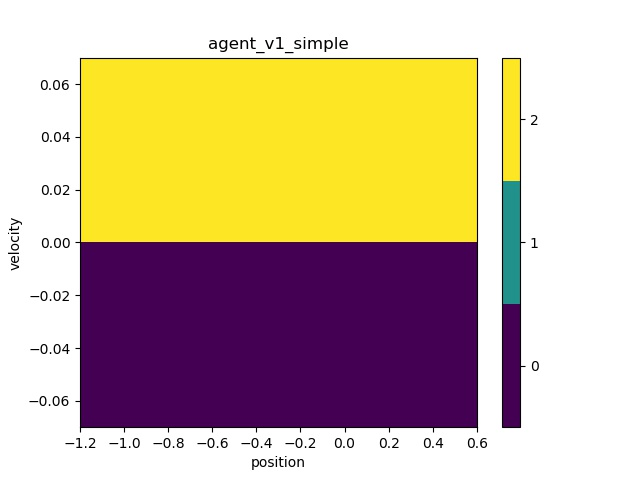
\includegraphics[width=.4\linewidth]{img/MTC/decision_plots/agent_v1_simple.jpg}
    \caption{A subfigure}
    \label{fig:subf1}
\end{figure}
\begin{figure}
    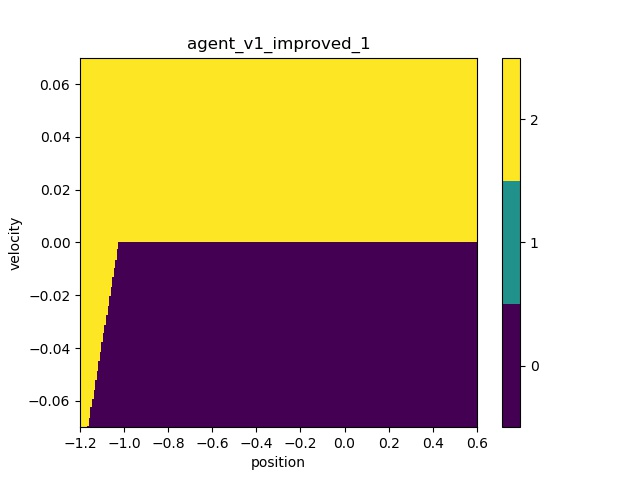
\includegraphics[width=.4\linewidth]{img/MTC/decision_plots/agent_v1_improved_1.jpg}
    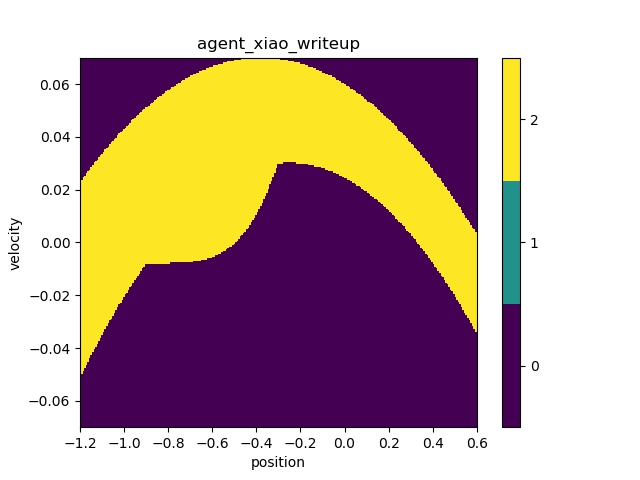
\includegraphics[width=.4\linewidth]{img/MTC/decision_plots/agent_xiao_writeup.jpg}
    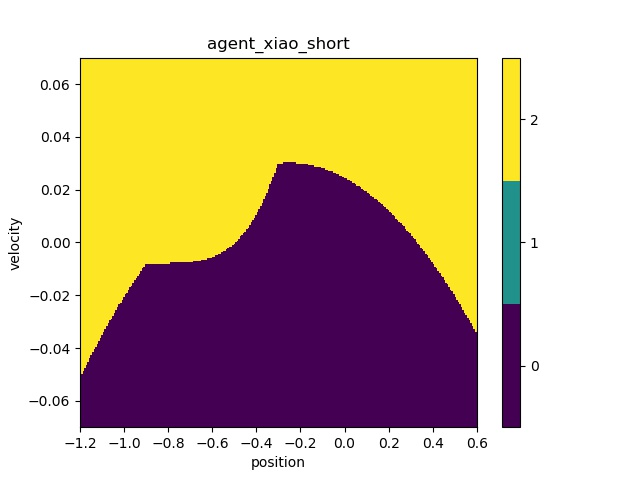
\includegraphics[width=.4\linewidth]{img/MTC/decision_plots/agent_xiao_short.jpg}
\end{figure}
\begin{figure}
    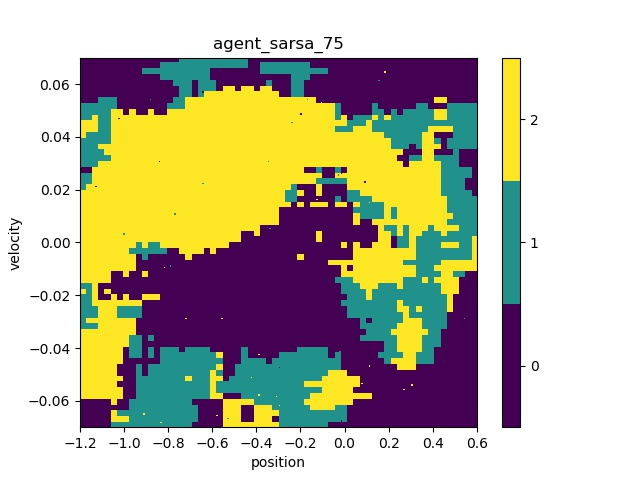
\includegraphics[width=.4\linewidth]{img/MTC/decision_plots/agent_sarsa_75.jpg}
    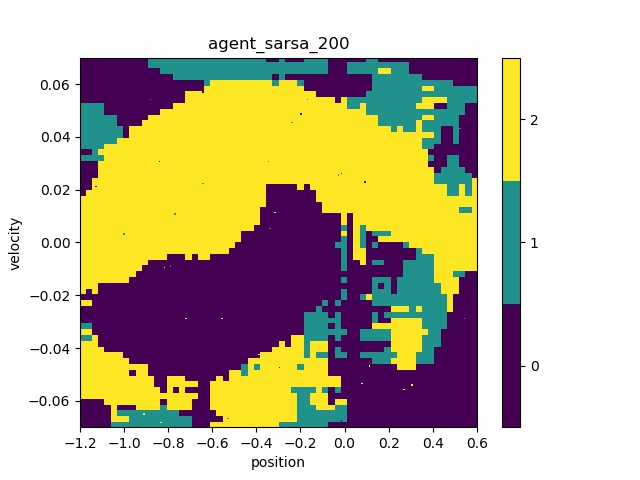
\includegraphics[width=.4\linewidth]{img/MTC/decision_plots/agent_sarsa_200.jpg}
    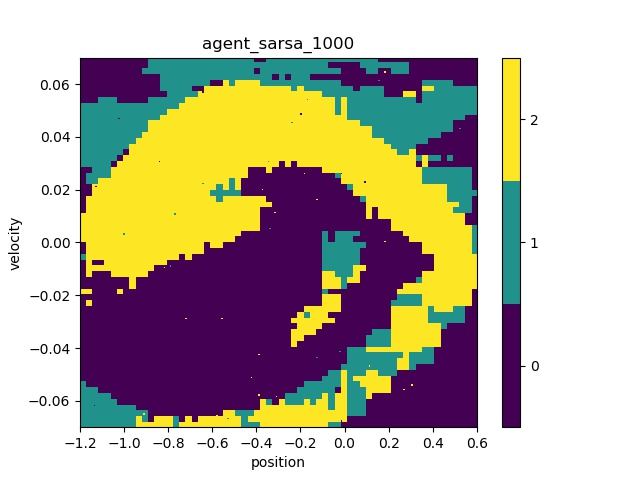
\includegraphics[width=.4\linewidth]{img/MTC/decision_plots/agent_sarsa_1000.jpg}
    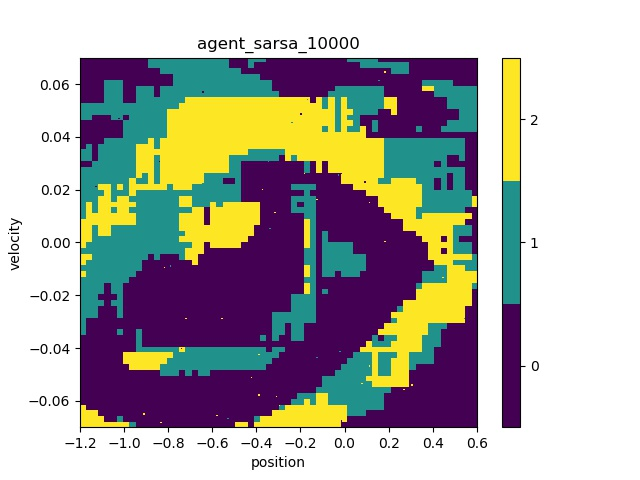
\includegraphics[width=.4\linewidth]{img/MTC/decision_plots/agent_sarsa_10000.jpg}
    \caption{Caption}
    \label{fig:my_label}
\end{figure}


\subsection{Reference programs}

The genetic improvement process was applied to numerous reference programs of which the following were thoroughly evaluated.

\begin{itemize}
    \item simple policy: ``Move towards the moving direction''
    \item simple fix: the simple policy with the decision for either 0 or 2 is not changeable by the genetic programming process
    \item simple fix extended: the simple policy with another if statement allowing to perform action ``no push'' aswell
    \item little expert: simple agent reversing earlier on the last turn
    \item true expert: compact but high end program that exceeds the fitness of sarsa75 
    \item closed policy: current lederboard leader
\end{itemize}


\subsection{fitness kernel fitting error regression [todo what name?]}

Mountain car's action space ${0, 1, 2}$ is ordered and scaled. The performance can therefore be calculated with some sort of regression kernel instead of only fitting result matches.

The action space further is one discrete dimension, leaving plenty of options to unitize the evaluation process:

\begin{itemize}
    \item one-hot encoding.
    
    All actions are one-hot encoded for which a softmax-probability is calculated [TODO softmax]. This does resemble the structure of a regular program though, what makes it difficult to use the tree edit distance.
    
    \item Return the action as part of the gp-process evaluation. If a value is not discrete, a value must be assigned.
\end{itemize}

The following regression kernels were evaluated for their suitability.
\begin{itemize}
    
    %\item match: counting the amount of perfect fits. 
    %The match-kernel suits very well for categorical data results such as fitting names, animals or cities. 
    \item The action space has a minimum and maximum value. If the program calculates values out of this bound, they should be interpreted as if the bias towards this decision is ``stronger'' , making the maximum difference $2$.  where values larger or smaller should not be punished.
    \item maximum penalties. trying to reduce the large amount of 
    \item simulate evaluation process by assigning values to action space. Every continuous result gets assigned to the closest action. The functions hiding behind this last step is kind of hidden. Small improvements can not be made easily, as it is only discovered when at least one point gets assigned correctly.
    \item only punish wrong decisions with regression
    \item simulate evaluation with a small regression penalty
\end{itemize}
ghu

The genetic programming process without fix nodes has the advantage that optimisations can be made easier.

\subsection{Analysing results, visualizing results}

The mountain car problem is very clear with only two dimensions, which opens up many possibilities for clear graphics.
A widespread visualization of the mountaincar problem is the decision plot, on which you can see the selected actions of the agent for the whole state space as a 2d-grid.
The x-axis is the position and the y-axis as speed, the actions are divided by colors.

[TODO Images, Analysis Images]

However, the relevant state space is much smaller. A functioning agent only comes into states that are arranged in a snail-like fashion as seen in [todo ref].

[TODO images]

Since two agents are to be compared, the same plot can also be visualized as a plot of decision differences. Again, the plot can be limited to the areas that are actually reached by the agent.

[TODO Images]

\section{Mountain car experiments}

\subsection{simple binary + SARSA 75, fix nodes}

Improving the simple binary approach leaves the genetic programming w











Problems with mountain car experiments
\begin{itemize}
    \item Change of sign
    \item change of sign at weird spots
    \item Parameter range (should they be normalized?)
    \item Not enough samples for small improvements?
    \item Unstable sarsa?
    \item Outlier can be found easier
    \item Difference 2-1 and 0-1 is the same, although completely different actions
    \item Fast moving car vs slowly moving generate different amount of data per area. coarse data can be fit better than dense data.
\end{itemize}